\chapter{Upgrade of the Upstream Tracker}
\label{ref:ut}

Located in the fringing fields in front of the LHCb dipole Magnet,
the Upstream Tracker (UT) plays an important role in improving the tracking
quality and speeding up trigger decisions:
Combining hits from VELO, SciFi, and UT provides the best \pt resolution
and reduce the rate of random combinations from VELO and SciFi to form
ghost tracks to about one fourth.
Furthermore, combining hits from VELO and UT removes low-\pt tracks and narrows
down the hit search window in SciFi, allowing for a faster track reconstruction
which leads to faster trigger decisions.

The University of Maryland group is responsible for the design, testing, and
commissioning of the peripheral and power regulating electronics;
An overview of the UT, discussed in \cref{ref:ut:overview},
summarizes the specifications and utilities of these electronics,
together with the sensors.
The author is tasked to test and develop quality assurance procedure for
the Data Control Board (DCB),
part of the peripheral electronics,
which is responsible to concentrate sensor readout and to control the UT
detector;
more details on DCB is described in \cref{ref:ut:dcb}.
In doing so, the author gained understanding on the data acquisition and control
system of the UT;
a review of these systems are summarized in \cref{ref:ut:daq} and
\cref{ref:ut:ctrl}, respectively.


\section{Overview of the UT detector}
\label{ref:ut:overview}

The UT consists of 4 planar detection layers with full LHCb acceptance coverage.
As shown in \cref{fig:ut-layers},
the first and last layers are vertical,
whereas the second and third are rotated by a stereo angle of $\pm 5^\circ$
to form a $x$-$u$-$v$-$x$ configuration.
The vertical planes provide highest hit resolution in the bending plane
($x$-$y$);
the rotated planes provide a measurement in the non-bending direction ($z$).

\begin{figure}[!htb]
    \centering
    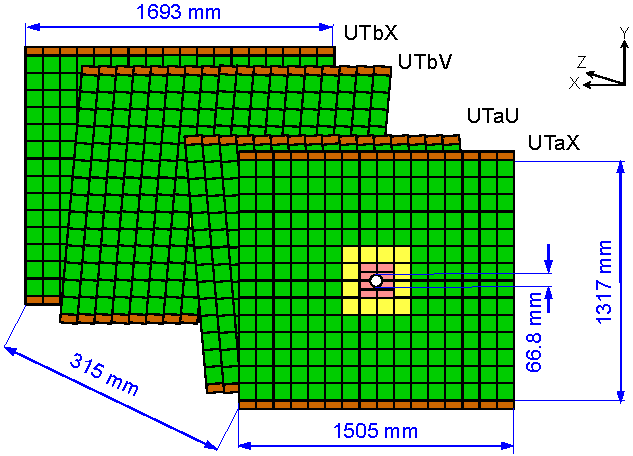
\includegraphics[width=0.7\textwidth]{./figs-lhcb-upgrade-overview/tracking/ut_upgrade.pdf}
    \caption{
        Four detection layers of UT,
        arranged in a $x$-$u$-$v$-$x$ configuration.
    }
    \label{fig:ut-layers}
\end{figure}

Each detection layer is made of a number of staves,
a vertical strip of sensors and their readout electronics;
the staves are discussed in \cref{ref:ut:overview:stave}.
The sensor readouts are collected by the electronics hosted inside Peripheral
Electronics (PEPI) crates at the top and bottom of the detection layer,
and are described in \cref{ref:ut:overview:pepi}.
To reduce radiation damage, the low voltage regulators (LVRs),
which supply power to the detector electronics,
are placed further away from the beam at the service bay;
a brief description of the LVR is given in \cref{ref:ut:overview:lvr}.
An overview of the UT exterior is provided in \cref{fig:ut-exterior}.

\begin{figure}[!htb]
    \centering

\begin{tikzpicture}
    \node [anchor=south west] (main) {
        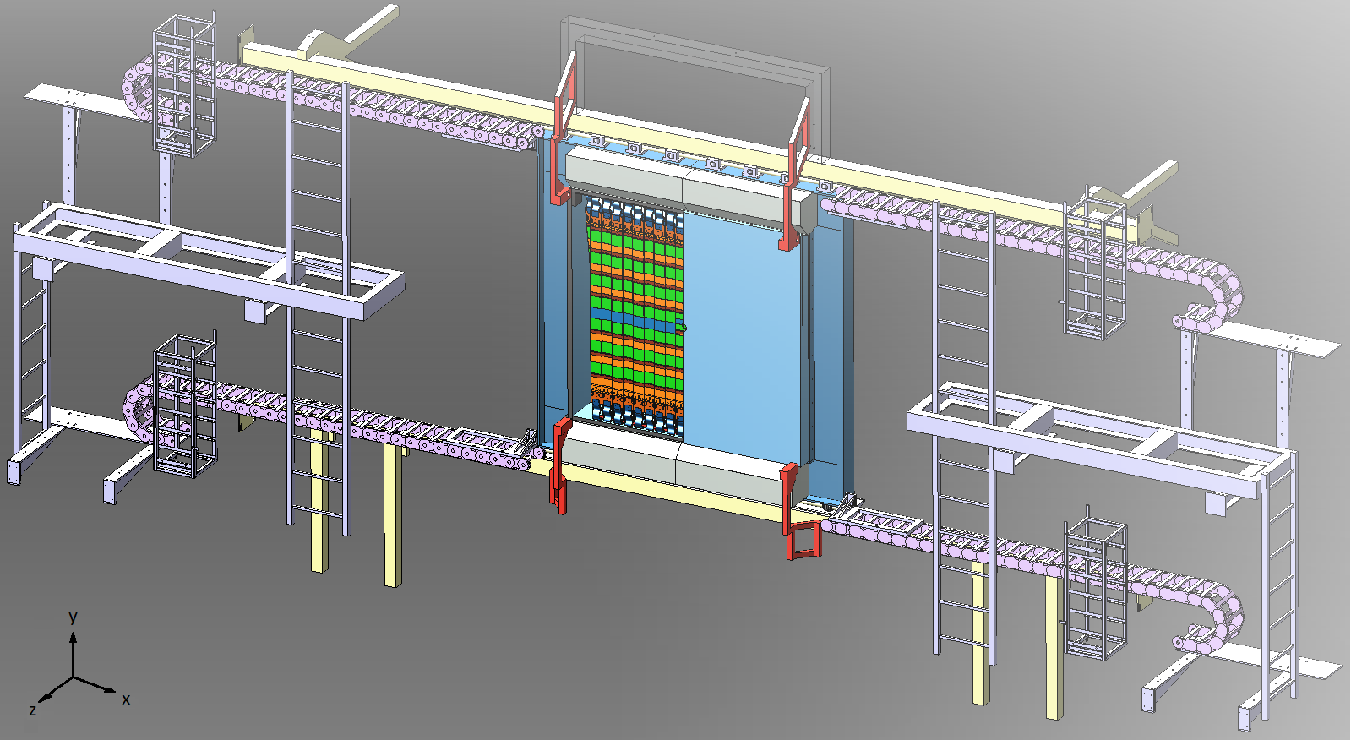
\includegraphics[width=0.88\textwidth]{./figs-ut-upgrade/detector/ut_exterior.pdf}
    };
    \begin{scope}[x=(main.south east),y=(main.north west)]
        \node[text=black] (A) at (0.7,0.92) {\textbf{PEPI}};
        \node (B) at (0.5,0.73) {};
        \draw[->, thick, draw=black, to path={-| (\tikztotarget)}] (A) edge (B);

        \node[text=black] (C) at (0.3,0.14) {\textbf{Detector box}};
        \node (D) at (0.52,0.52) {};
        \draw[->, thick, draw=black, to path={-| (\tikztotarget)}] (C) edge (D);

        \node[text=black] (E) at (0.7,0.8) {\textbf{Service bay}};
        \node (F) at (0.82,0.74) {};
        \draw[->, thick, draw=black, to path={-| (\tikztotarget)}] (E) edge (F);
    \end{scope}
\end{tikzpicture}

    \caption{
        UT exterior in the LHCb cavern.
        Taken from \cite{Andrews:2018vla}.
    }
    \label{fig:ut-exterior}
\end{figure}


\subsection{Stave}
\label{ref:ut:overview:stave}

Illustrated in \cref{fig:ut-layers} as a vertical strip,
supported by a carbon fiber core with CO$_2$ cooling pipes,
a stave consists of 4 flexible cables (2 on each side) with sensors and hybrid
readout wire-bonded on each flex.
Shown in \cref{fig:stave}, the front and back sensors are mounted with an
overlap to ensure coverage.

\begin{figure}[!htb]
    \centering
    \begin{subfigure}[t]{0.48\textwidth}
        \centering
        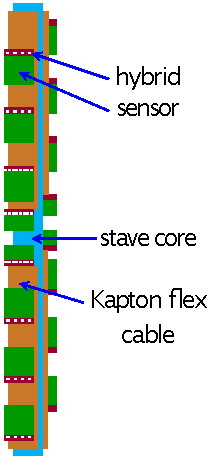
\includegraphics[height=20em]{./figs-ut-upgrade/detector/ut_stave.pdf}
        \caption{
            Schematic of a UT stave.
            Each side of a stave contains two Kapton flex cables.
        }
    \end{subfigure}
    \hspace{10pt}
    \begin{subfigure}[t]{0.48\textwidth}
        \centering
        \includegraphics[width=20em,angle=90]{./figs-ut-upgrade/detector/ut_stave_flex_cable.pdf}
        \caption{
            A signal and power layer of the Kapton flex cable.
            The low voltage coppers are shown in green;
            the data and high voltage lines are in red.
        }
    \end{subfigure}

    \caption{
        UT stave.
    }
    \label{fig:stave}
\end{figure}

There are four types of sensors with different specifications.
The sensors close to the beam pipe (yellow and pink in \cref{fig:ut-layers})
have a finer pitch of 93.5~$\upmu$m and are made with \emph{n-in-p} process for
more radiation hardness,
mainly due to concerns on occupancy and radiation damage.
In addition, the eight half-height sensors (pink) have their strip length halved
to further improve resolution near the beam pipe,
with the four sensors immediately surrounding the pipe having
circular cutouts, instead of rectangular gaps as in TT, to ensure maximum
coverage in the very forward direction.
The outer sensors (green) have a coarser pitch of 187.5~$\upmu$m fabricated with
\emph{p-in-n} technology to reduce cost
\cite{Carli:2783293}.

To minimize the transmission path of the analogue sensor output, readout
SALT ASICs\footnote{
    SALT is developed by the UT collaboration.
    ``ASIC'' stands for Application-Specific Integrated Circuit.
} are glued to a ceramic stiffener along with a sensor and electronic hybrid
circuit to form a single UT module.
The sensor strips are wire-bonded to the input pins of the SALT\footnote{
    SALT ASICs are represented by small white rectangles in
    \cref{fig:ut-layers}.
}
\cite{Wang:2015mem}.
A sample UT module is shown in \cref{fig:ut-module}.

\begin{figure}[!htb]
    \centering
    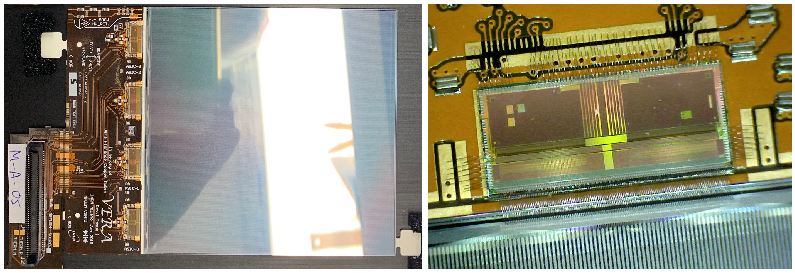
\includegraphics[width=0.9\textwidth]{./figs-ut-upgrade/detector/ut_sensor_module.pdf}
    \caption{
        (Left) Module built from type A sensor with a hybrid circuit carrying
        4 SALT ASICs.
        (Right) A SALT ASIC, glued on a hybrid, with its inputs wire-bonded
        to a type A sensor.
        Taken from \cite{Carli:2783293}.
    }
    \label{fig:ut-module}
\end{figure}

Fabricated with TSMC 130~nm CMOS process, SALT is capable of extract, shape,
and digitize analogue signals from the sensor at 40~MHz from 128 channels
simultaneously.
It requires an external 40~MHz clock signal,
which it locks on via a phase-lock loop (PLL),
to work.
It is also capable of generating pseudo-random test patterns on its own without
any excitation on the sensor, which comes handy in testing the data transmitting
quality for the DCB.
As an ASIC, SALT has limited configurability by writing registers via the I2C
protocol \cite{s22010107}.


\subsection{PEPI}
\label{ref:ut:overview:pepi}

Peripheral electronics (PEPI) are responsible for dispatching power to SALTs,
aggregating readout from SALTs to the counting room,
and propagating control commands to the front-end electronics\footnote{
    Front end electronics refer to SALTs and DCBs, which sit close to the beam.
}.
A diagram for data readout and control signal propagation in the UT is displayed
in
\cref{fig:ut-readout-diagram}.

\begin{figure}[!htb]
    \centering
    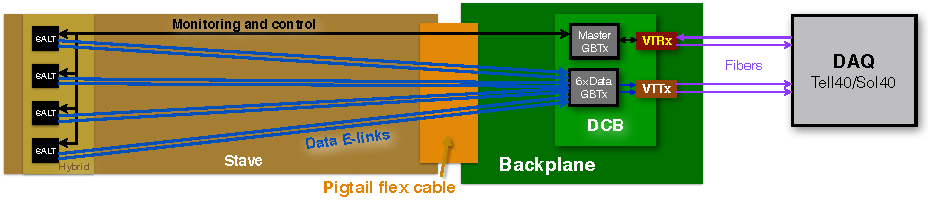
\includegraphics[width=0.85\textwidth]{./figs-ut-upgrade/detector/ut_data_control_flow.pdf}
    \caption{
        UT data and control signal flow diagram.
    }
    \label{fig:ut-readout-diagram}
\end{figure}

Due to space constraint, power, readout data, and control command
are all \emph{dispatched} by a board named Backplane (BP).
Each BP is connected to up to 12 Staves via the Pigtail flex cable,
an engineering marvel on its own\footnote{
    More details regarding the Pigtail can be found in
    \cite{Andrews:2018vla}.
    It is worth noting that during the detector installation,
    very precise bending of the Pigtails are needed to ensure good connectivity.
},
which dispatches power, data, and control signals between the BP and SALTs on
the stave in an \emph{extremely} limited space.
A BP can also host up to 12 DCBs.
Each DCB then serialize its input data and convert the digitized electronic
signal to an optic one which is sent to the counting room via fibers.
DCB is also responsible for receiving and translating control commands from the
counting room to both itself and SALT ASICs.
In other words, the whole configurable part of the UT detector is exposed as DCB
registers to the counting room.

PEPI are hosted in PEPI crates, with each containing a single Backplane and up
to 12 DCBs,
as can be seen in \cref{fig:pepi-crate}.
The crate is also responsible for cooling and providing a common ground
reference for all SALTs and DCBs.

\begin{figure}[!htb]
    \centering
    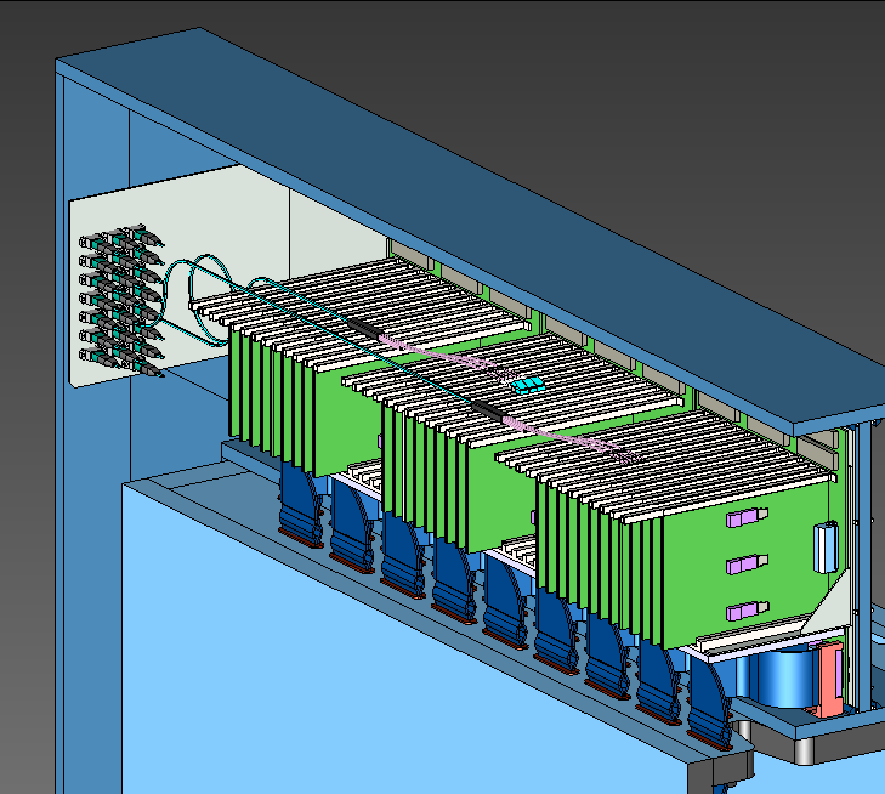
\includegraphics[width=0.7\textwidth]{./figs-ut-upgrade/detector/pepi_crates.pdf}
    \caption{
        A schematic drawing of 3 PEPI crates with DCBs and Pigtails plugged in.
        Taken from \cite{Andrews:2018vla}.
    }
    \label{fig:pepi-crate}
\end{figure}

Backplanes are nothing but a (huge) net of microscopic cables delivering power
and facilitating data exchange to specific connector pins, and contain no active
component (i.e. integrated circuit).
While conceptually simple, Backplanes are extremely hard to route because the
trace density is extremely high.
Fabricated with 28 layers of PCBs\footnote{
    As a reference, a typical motherboard for a desktop PC has 6 layers of PCBs.
}, BPs are at the limit of manufacturability.
To ensure that the traces are routed correctly,
the connectivity map (referred as a ``netlist'') is exported to a
machine-parsable language\footnote{
    One such option exports the netlist to a language that is compatible with
    Common Lisp.
} and checked against a set of pre-defined rules, for example DCBs and
SALTs have differing voltage requirements,
by a Python script.

\begin{figure}[!htb]
    \centering
    \begin{subfigure}[t]{0.48\textwidth}
        \centering
        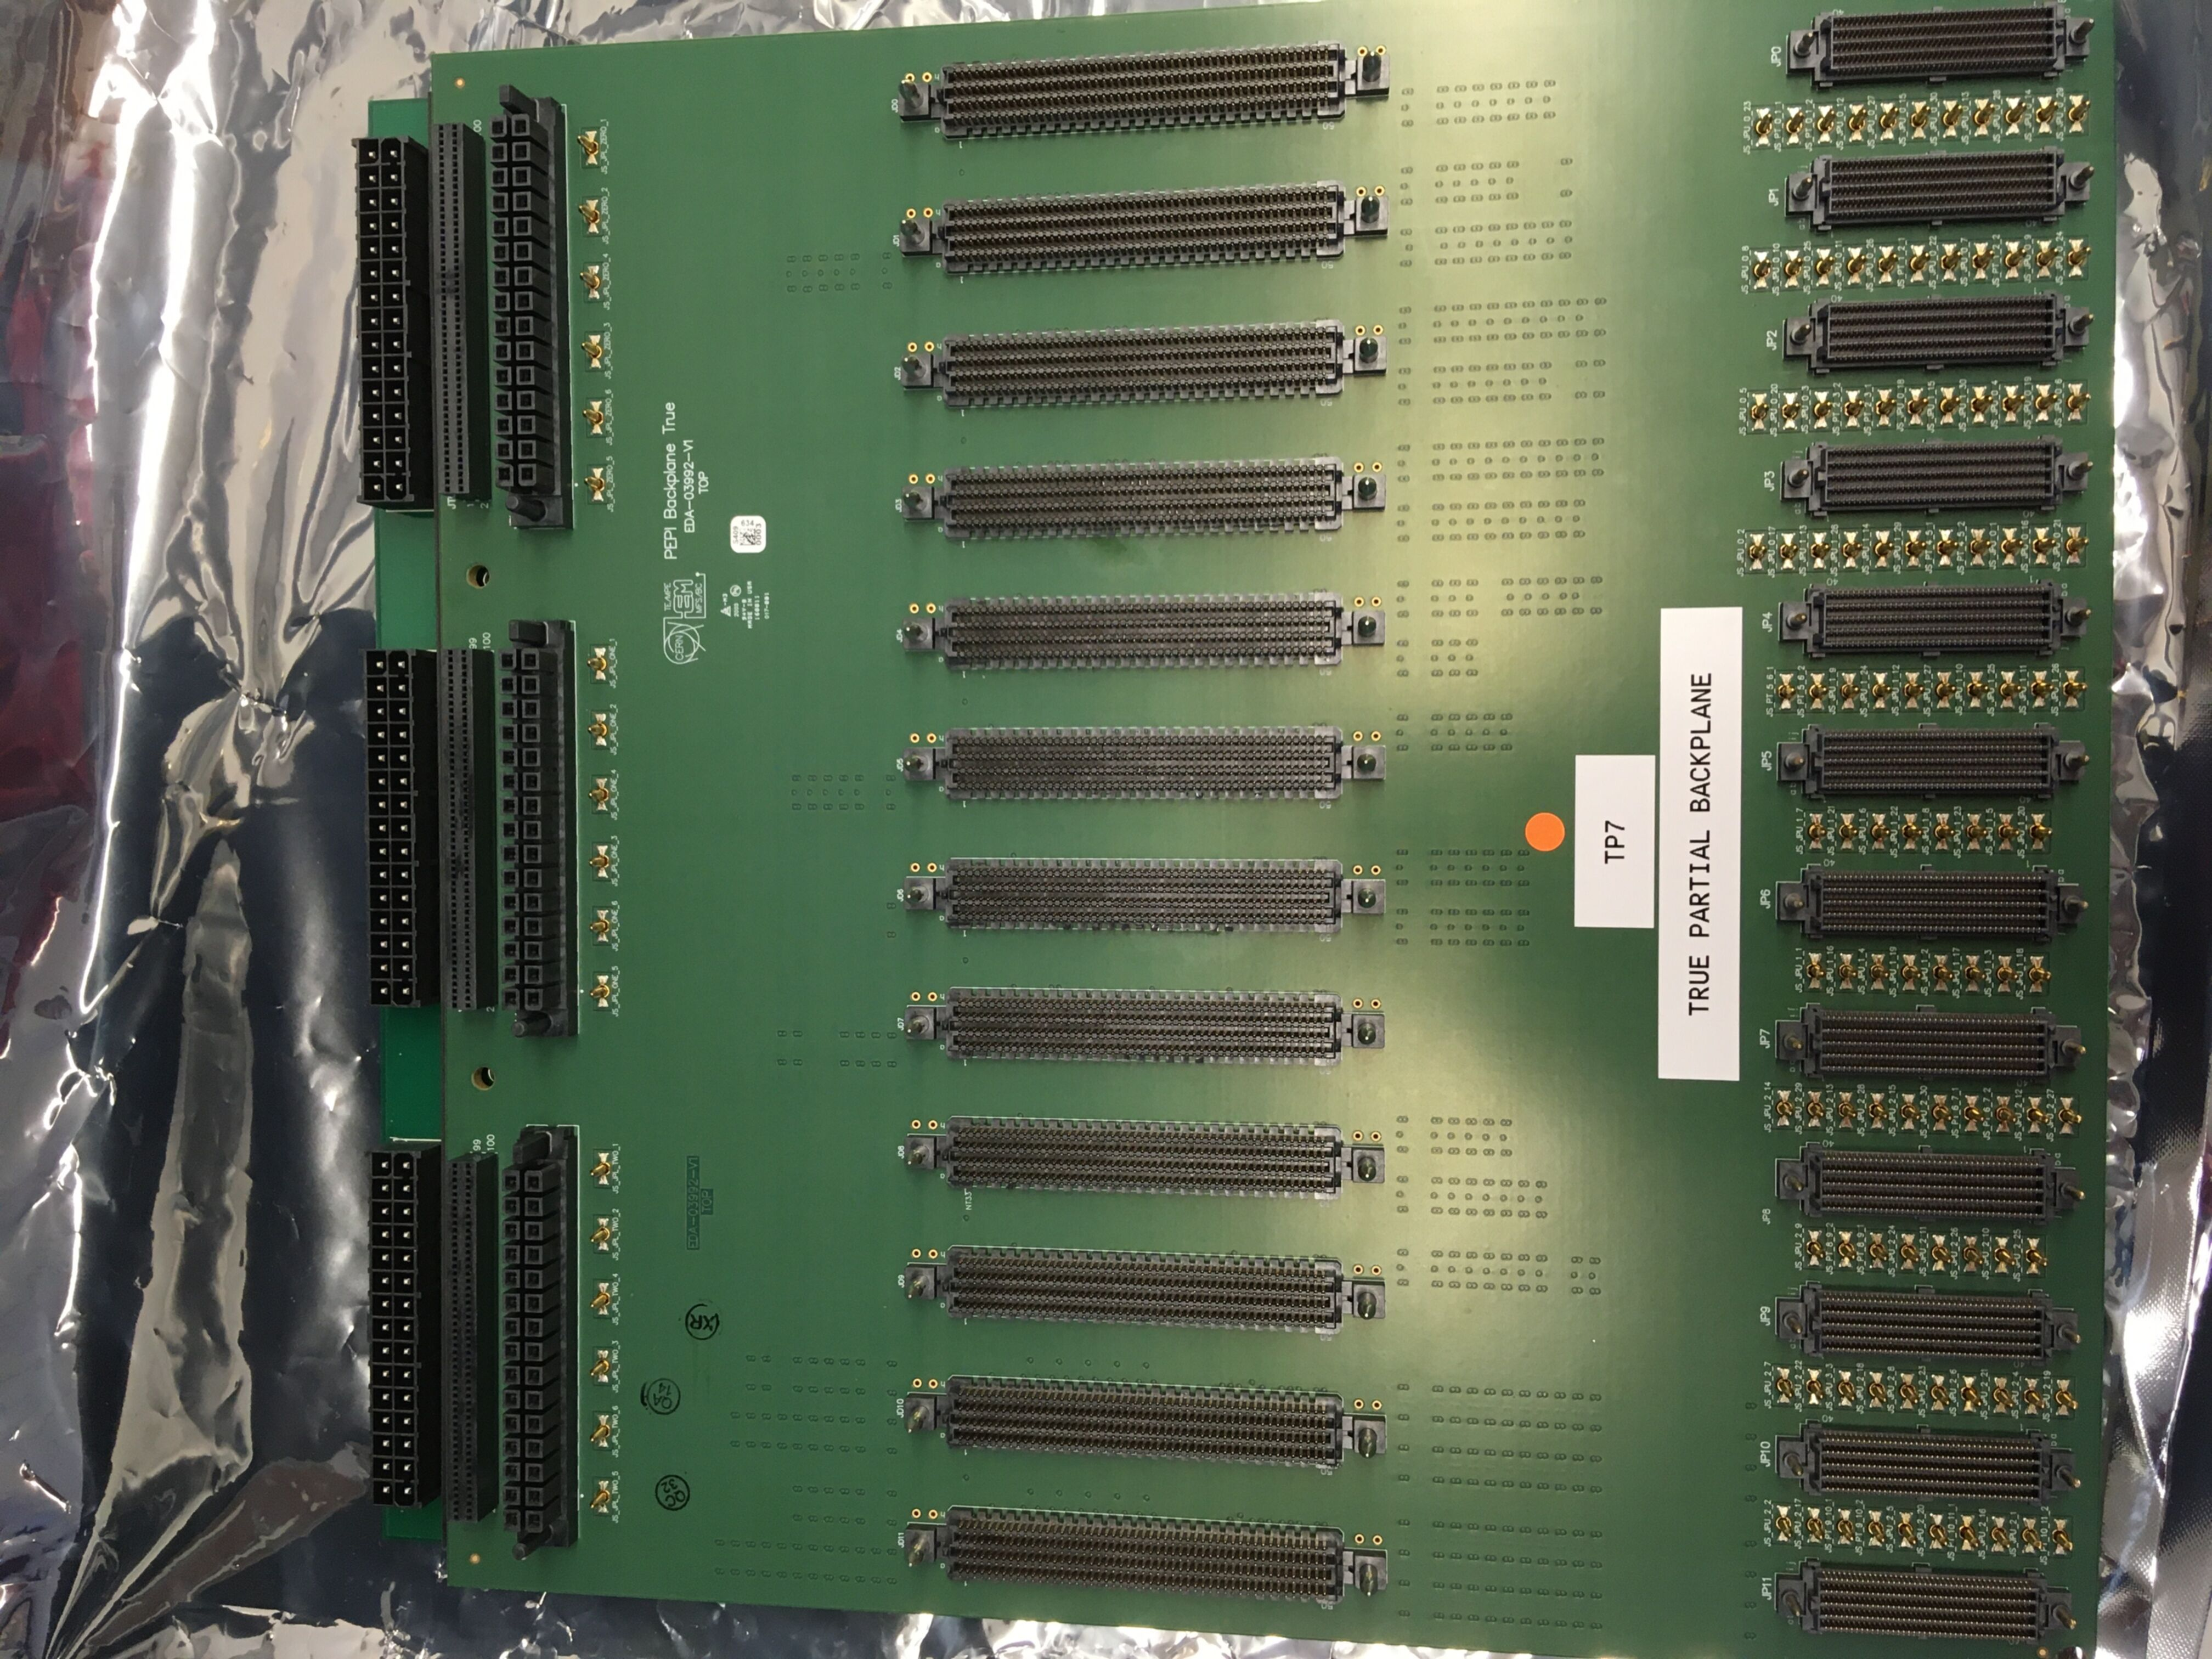
\includegraphics[height=20em]{./figs-ut-upgrade/detector/backplane_compressed.jpg}
        \caption{
            A production Backplane.
        }
    \end{subfigure}
    \hspace{10pt}
    \begin{subfigure}[t]{0.48\textwidth}
        \centering
        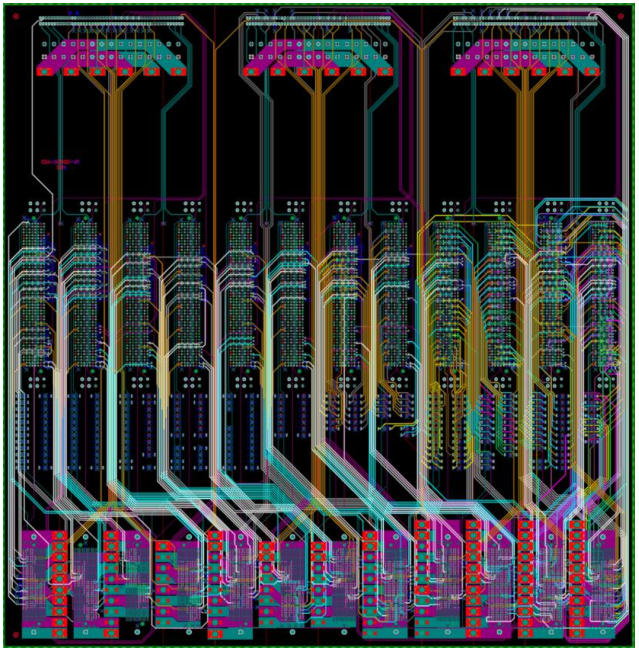
\includegraphics[height=20em]{./figs-ut-upgrade/detector/backplane_trace.pdf}
        \caption{
            Traces of the backplane are of ultra high density.
        }
    \end{subfigure}

    \caption{
        A production Backplane and its copper trace implement.
    }
    \label{fig:backplane}
\end{figure}

Data Control Board (DCB), shown in,
consists of a master GBTx ASIC
for production of a stable, low jitter\footnote{
    Deviation from the presumed clock frequency.
} clock from the clock signal provided by the readout system in the counting
room via a bi-direction optical link,
and distribution of clock signal to 6 data GBTxs and all connected SALTs,
hereby referred as ``downstream ASICs''\footnote{
    This name is invented by me.
    ``Downstream'' refers to the fact that these ASICs take the clock
    distributed by the master as their reference clock.
};
6 data GBTxs operate in simplex transmitter mode to
serialize, prepare in a way suitable for optical transmission,
and convert the SALT readouts to optical signal via the GigaBit Laser Drive
(GBLD) ASIC which then transmits the readout via optical links;
A GBT-SCA ASIC, connected to master GBTx and downstream ASICs,
is responsible for relaying slow control commands (e.g. I2C) and telemetry
(e.g. thermistor readout on SALT via its built-in ADC) between downstream ASICs
and the control system of the detector.

As the author spent quite some time to test (and to make sense) of the
DCBs, more information regarding DCBs will be provided in \cref{ref:ut:dcb}.


\subsection{LVR}
\label{ref:ut:overview:lvr}


\section{The Data Control Board (DCB)}
\label{ref:ut:dcb}


\section{Data acquisition in UT}
\label{ref:ut:daq}


\subsection{TELL40 the event builder}


\subsection{Timing and Fast Control (TFC)}


\section{Control system of UT}
\label{ref:ut:ctrl}


